

\section{Preliminary experiments}\label{sec:setup}
In this Section, we describe two preliminary experiments we conducted in Spring 2018 following the conceptual framework presented in the previous section. The first experiments is a rehearsal between two musicians in the same room, where we insert visual occlusions to test their ability to interact in adverse conditions. The second experiments is a set of rehearsals between five couples of musicians in two separate rooms, connected via a network emulator to test the sense of presence and the quality of performance at different latency conditions. The results of the two experiments are discussed in the next section.


\begin{figure}[t]
	\centering
	\includegraphics[width=\columnwidth]{img/veli.eps}
	\caption{The two musicians in experiment 1, with partial occlusion and blurred effect.}
	\label{fig:veli}
\end{figure}

\subsection{Co-presence performance with visual occlusion}
We invited a string duo to make a pilot test of the environment, the perceptual questionnaire and the musical pieces that we intended to use for the second experiment. We also included a test on adverse conditions of the medium (visual occlusion) to qualitatively assess the importance of video feedback in NMPs.

We show a summary of the test conditions in Table \ref{tab:exp1}. The two subjects were a violin and a cello players and are brothers, they have a long-time experience playing together and use a wide set of visual and audio cues to interact. For the musical parts, we created a composition that requires mutual interaction and understanding. The composition includes attacks, alternate scales, changes of tempo, unison playing, sustained loop. The parts are described in detail in \cite{CIM2018} and publicly available\footnote{https://tinyurl.com/intermusicCIM2018}.


\begin{figure*}[t]
	\centering
	\begin{subfigure}[t]{.48\columnwidth}
		\centering        
		%\includegraphics[trim={.5cm 13.7cm 13.5cm .5cm},clip,width=\textwidth]{figures/ann1}
		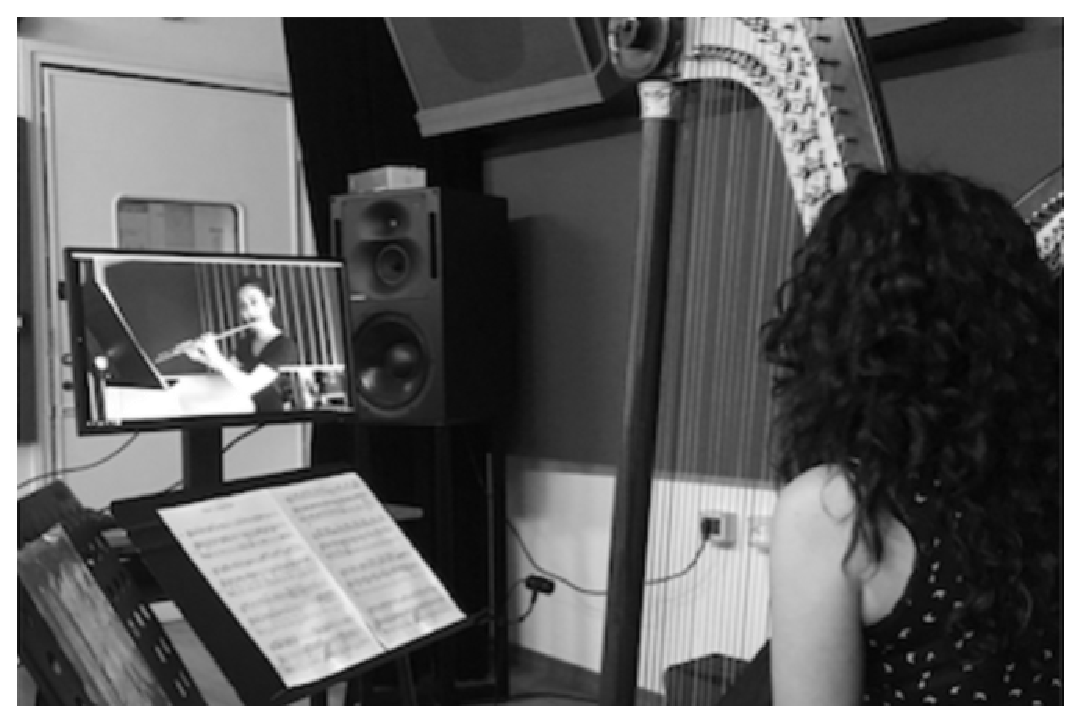
\includegraphics[width=\textwidth]{img/as.eps}
		\caption{A harp player performing in her real environment}
		\label{subfig:as}
	\end{subfigure}
	\begin{subfigure}[t]{.48\columnwidth}
		\centering        
		%\includegraphics[trim={.5cm 13.7cm 13.5cm .5cm},clip,width=\textwidth]{figures/ann1}
		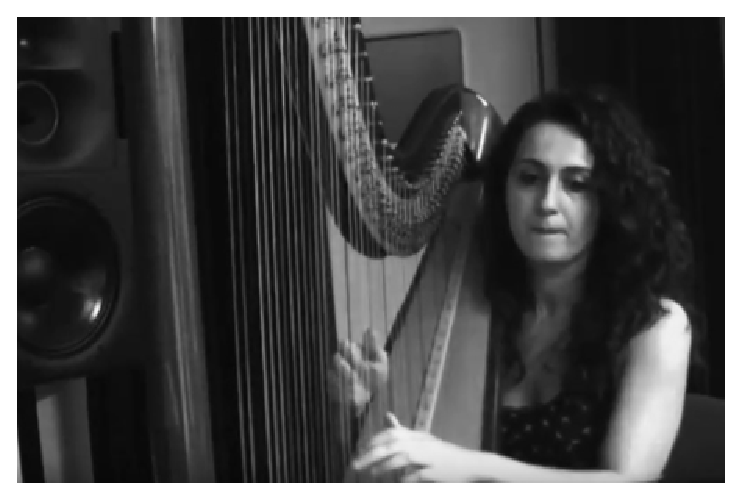
\includegraphics[width=\textwidth]{img/av.eps}
		\caption{A harp player as visually perceived in the virtual environment}
		\label{subfig:av}
	\end{subfigure}
	\begin{subfigure}[t]{.48\columnwidth}
		\centering        
		%\includegraphics[trim={.5cm 13.7cm 13.5cm .5cm},clip,width=\textwidth]{figures/ann1}
		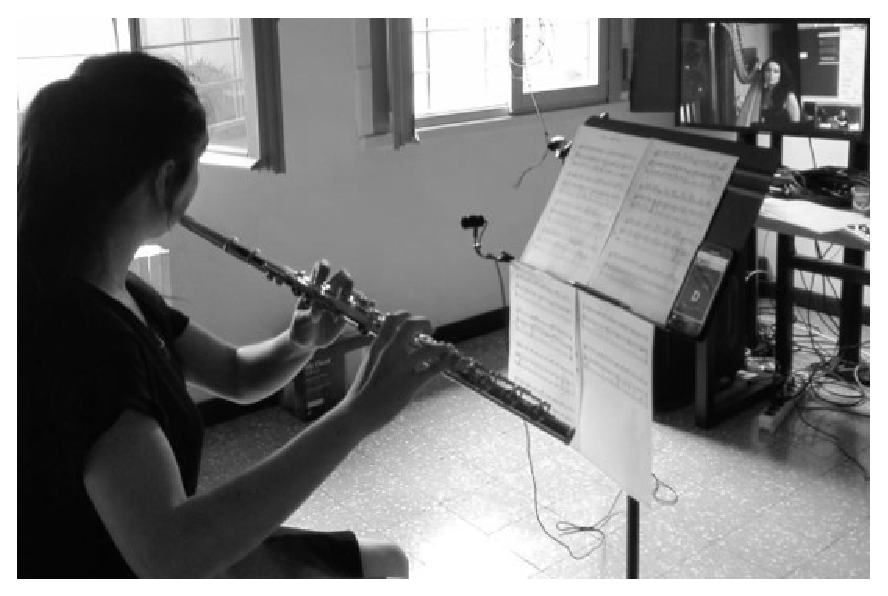
\includegraphics[width=\textwidth]{img/fs.eps}
		\caption{A flute player performing in her real environment}
		\label{subfig:fs}
	\end{subfigure}
	\begin{subfigure}[t]{.48\columnwidth}
		\centering        
		%\includegraphics[trim={.5cm 13.7cm 13.5cm .5cm},clip,width=\textwidth]{figures/ann1}
		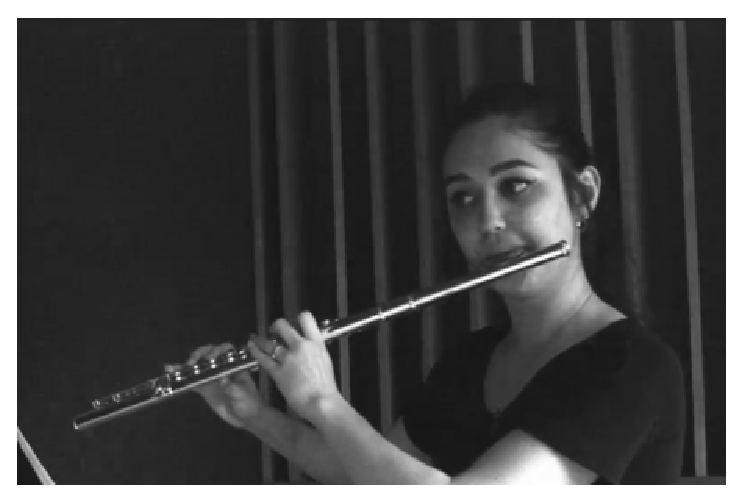
\includegraphics[width=\textwidth]{img/fv.eps}
		\caption{A flute player as visually perceived in the virtual environment}
		\label{subfig:fv}
	\end{subfigure}
	
	\quad 
	\caption{View of real environments and virtual environments in the networked experiment}\label{fig:afsv}
	
\end{figure*}

The performers were asked to play in two conditions: with no visual occlusion, and with partial visual occlusion, by inserting a tulle panel between the two instrumentalists, thus providing a blurring effect on their figures (as shown in Figure \ref{fig:veli}). The aim was to observe their behavior, adaptation strategies, and emerging non-verbal communication (bodily and musical gestures).

The data recording of the experiment was based on a subjective questionnaire on their sense of presence and free comments on the experience. 





\subsection{Sense of presence in NMPs}
Five couples of musicians, playing different combinations of instruments, took part in the experiment. The couples had familiarity in playing together since at least two weeks. The details of the experiment are reported in Tab.~\ref{tab:exp2}

Each session of the experiment comprised a single couple, the two musicians were placed in different rooms, standing in front of a screen, in order to be connected both with respect to video and audio. An example of the setup for the couple consisting of harp and flute players is shown in Fig.~\ref{fig:afsv}. In Fig.~\ref{subfig:as} and Fig.~\ref{subfig:fs} it is possible to see the viewpoints of the musicians consisting of the scores and the screens connected to the other room. 

The couples played the same parts considered in the previous experiments. The medium involved two computers equipped with LOLA connected through a network emulator, by means of which we could change the transmission latency. A single session consisted of the couple playing the same part in six repetitions, where each time we simulated a different latency level in a range between $28\mathrm{ms}$ and $134\mathrm{ms}$, as detailed in~\cite{CIM2018}. It is important to note that the latency levels weren't presented sequentially to the musicians (e.g. in a decreasing or increasing order), but were instead selected with no particular criterion for each repetition,.

We asked the musicians to fill two different subjective questionnaires. The first one was presented after each repetition and composed of five questions, selected in order to analyze their perception of the performance with respect to the latency just experienced. The second, reported in \cite{CIM2018}, was presented to the musicians at the end of the whole session and it consisted of 27 questions, investigating he various aspects of the experience such as their sense of presence and the peceived general quality of the performance.


\begin{table}[b]
	\centering
	\caption{Details of the NMP experiment. For a more in-depth description, we refer the reader to \cite{CIM2018} }
	\begin{tabular}{p{1.5cm}p{6cm}}
		\hline
		\textbf{Entity} & \textbf{Properties} \\
		\hline
		\textbf{Performance} & Five NMP performances. \newline  Parts arranged from Bartok pieces. \\
		\textbf{Subjects} & Five couples of musicians with different combinations of instruments. Average age: 21.9 years. Musical experience: at least 5 years\\
		\textbf{Environment} & Two rooms: two mastering studios in the Conservatory of Milan; acoustically equipped with bass traps. Musicians sit in front of a screen and a webcam and monophonic audio input/output.\\
		\textbf{Medium} & Software LOLA with video and audio transmission. Network emulator with different latency condition and fixed jitter. \\
		\textbf{Data} \newline \textbf{recording} & Audio recording of the performance from one room, audio/video recording using LOLA; perceptual questionnaire.\\
		\hline
	\end{tabular}
	\label{tab:exp2}
\end{table}



